% !TEX root = ../../main.tex

\subsection{Water adsorption}

The shape of the water vapour isotherm will be an indication of the hydrophilicity
of the material. By itself, alumina is a hydrophilic substance, with a contact 
angle of \SI{10}{\degree}. It is expected that the addition of the binder will
therefore increase the affinity of the resulting pellet towards water.

Looking at the resulting adsorption measurements one can see the typical downwards
shift of the pellet isotherms resulting from structure degradation. However, changes
in the interaction of the MOF with water do not seem to be highlighted. The low relative
pressure region (\(p/p^0 < 0.3\)) should be particularly indicative of any such 
changes, but an almost complete overlap can be seen in this region.
In particular, the UiO-66(Zr) isotherms have a surprising amount of similarity,
considering the loss of capacity seen in \ce{N2} physisorption and room temperature 
adsorption experiments.

It can be therefore concluded that overall, the addition of alumina has not influenced 
the behaviour towards water for the materials studied. The full water adsorption isotherms
can be found in Figure~\ref{fgr:shaping:wateradsorption}.

\begin{figure}[p!]
    \centering

    \begin{subfigure}{\linewidth}
        \centering
        \parbox{0.1\linewidth}{\caption{}\label{fgr:shaping:wateruio66}}%
        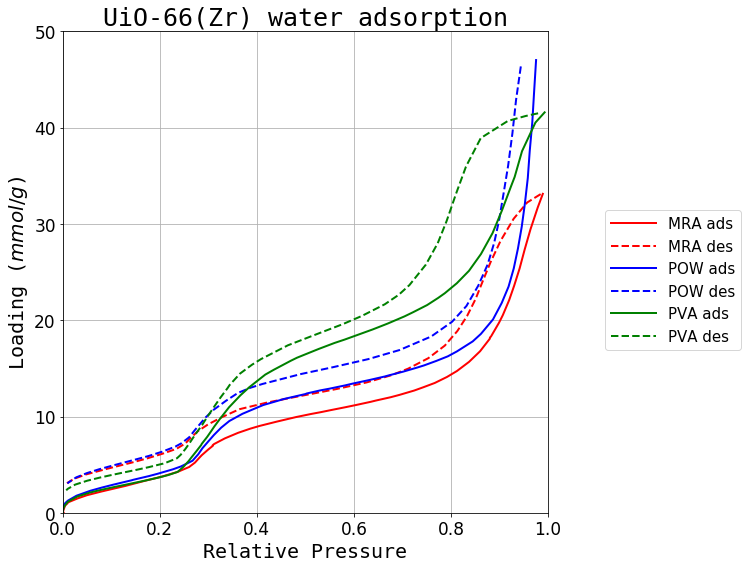
\includegraphics[width=0.3\textwidth]{water/UiO-66(Zr)-water}%
        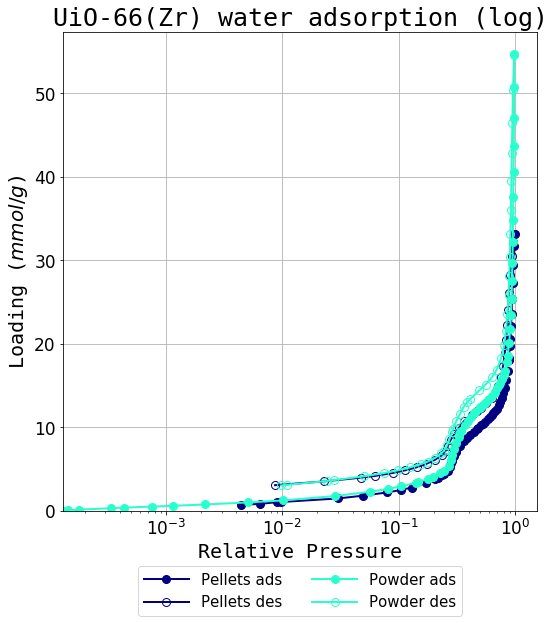
\includegraphics[width=0.3\textwidth]{water/UiO-66(Zr)-water-log}%
    \end{subfigure}

    \begin{subfigure}{\linewidth}
        \centering
        \parbox{0.1\linewidth}{\caption{}\label{fgr:shaping:watermil100}}%
        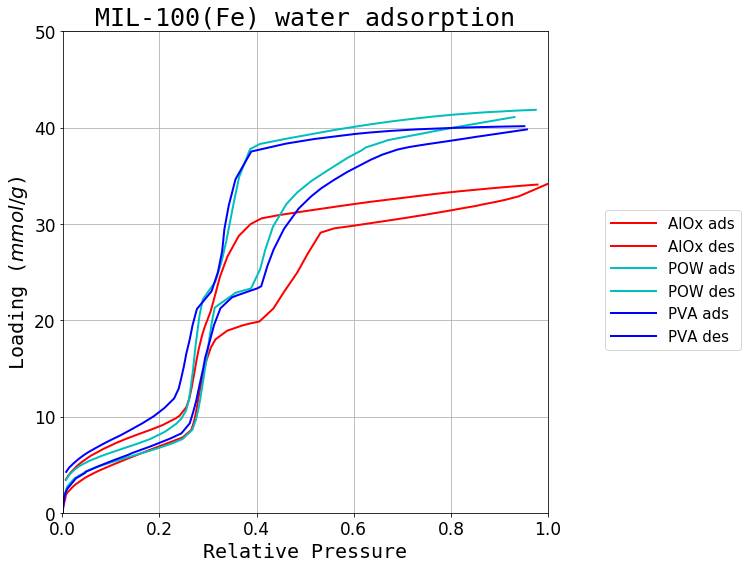
\includegraphics[width=0.3\textwidth]{water/MIL-100(Fe)-water}%
        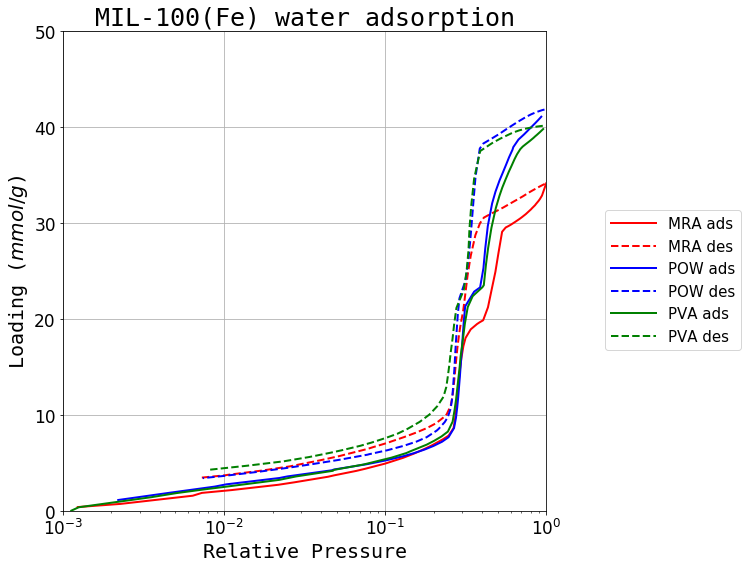
\includegraphics[width=0.3\textwidth]{water/MIL-100(Fe)-water-log}%
    \end{subfigure}

    \begin{subfigure}{\linewidth}
        \centering
        \parbox{0.1\linewidth}{\caption{}\label{fgr:shaping:watermil127}}%
        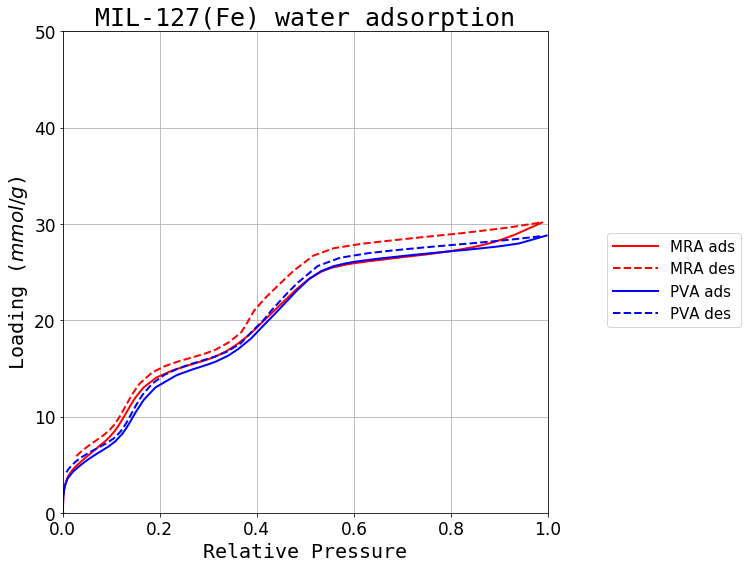
\includegraphics[width=0.3\textwidth]{water/MIL-127(Fe)-water}%
        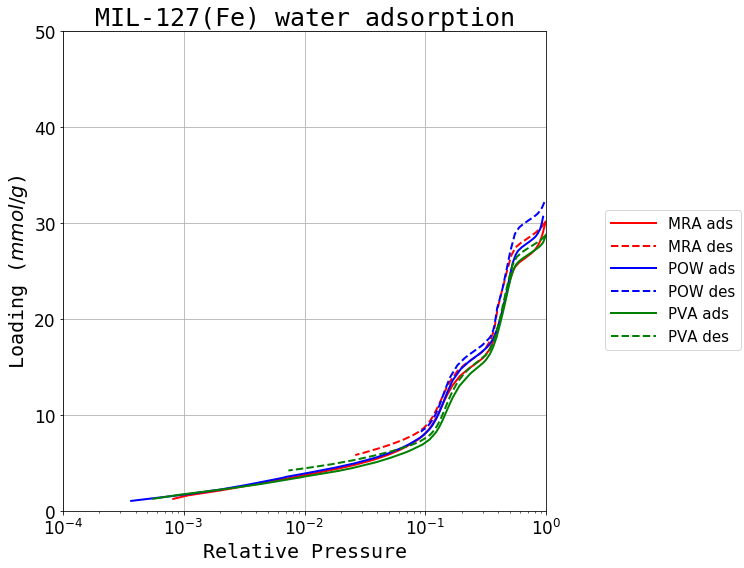
\includegraphics[width=0.3\textwidth]{water/MIL-127(Fe)-water-log}%
    \end{subfigure}
    
    \caption{Water adsorption isotherms (a) UiO-66(Zr), 
    (b) MIL-100(Fe) and (c) MIL-127(Fe). The powder sample is in light
    blue while the \(\rho\)-alumina sample in dark blue. Logarithmic
    graphs of the isotherms are on the right for clarity of the low
    pressure region.}%
    \label{fgr:shaping:wateradsorption}
\end{figure}